\documentclass{beamer}
\usetheme{Boadilla}
\usepackage{subfigure}

\begin{document}

\begin{frame}
\frametitle{Beta prior, binomial likelihood}
\begin{equation}
\theta\sim\textup{Beta}(1,1)
\end{equation}
\begin{equation}
X|\theta\sim\textup{Bin}(12,\theta)
\end{equation}
\begin{equation}
\theta|X=2\sim\textup{Beta}(3,11)
\end{equation}
\pause
\begin{block}{ABC Algorithm}
\begin{itemize}
  \item Sample $\theta\sim\textup{Beta}(1,1)$
  \item Sample $X|\theta\sim\textup{Bin}(12,\theta)$
  \item Accept $\theta$ if $X|\theta = 2$, otherwise reject.
\end{itemize}
\end{block}
\end{frame}

\begin{frame}
\frametitle{Beta prior, binomial likelihood}
\begin{figure}
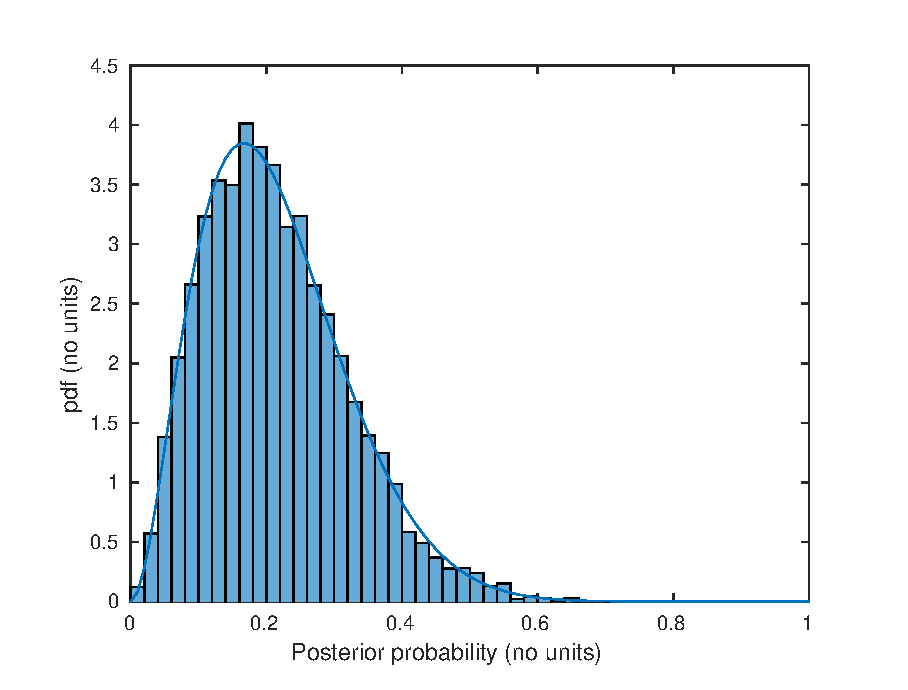
\includegraphics[width=0.5\textwidth]{binomial_ABC0528.eps}
\caption{10,000 samples using ABC.}
\label{binomial}
\end{figure}
$p$ value for $\chi^2$ goodness of fit test $(50\pm30)\%$ \\
$(10\pm10)$ rejects per accepted sample
\end{frame}

\begin{frame}
\frametitle{Normal-gamma prior, Normal likelihood}
\begin{block}{Prior}
\begin{equation}
\tau\sim\textup{Gamma}(\alpha_0,\beta_0)
\end{equation}
\begin{equation}
\mu|\tau\sim\textup{N}\left(\mu_0,1/(\nu_0\tau)\right)
\end{equation}
\end{block}
\pause
\begin{block}{Likelihood}
\begin{equation}
X|\mu,\tau\sim\textup{N}(\mu,1/\tau)
\end{equation}
\end{block}
\pause
\begin{block}{Joint Posterior}
\begin{equation}
\mu,\tau|X\sim\textup{NGamma}
\left(
	\mu_1,
	\nu_1,
	\alpha_1,
	\beta_1
\right)
\end{equation}
\end{block}

\end{frame}

\begin{frame}
\frametitle{Normal-gamma prior, Normal likelihood}
\begin{block}{Marginal Posterior}
\begin{equation}
\mu|X = \sqrt{\dfrac{\beta_1}{\alpha_1\nu_1}} T_{2\alpha_1}
+ \mu_1
\end{equation}
and
\begin{equation}
\tau|X \sim \textup{Gamma}\left(
\alpha_1,\beta_1
\right)
\end{equation}
where $T_{2\alpha}\sim t_{2\alpha}$.
\end{block}
\end{frame}

\begin{frame}
\frametitle{Normal-gamma prior, Normal likelihood}
\begin{block}{ABC Algorithm}
\begin{itemize}
	\item Sample $\tau\sim\textup{Gamma}(\alpha_0,\beta_0)$
	\item Sample $\mu|\tau\sim\textup{N}\left(\mu_0,1/(\nu_0\tau)\right)$
	\item Sample $n$ times $Y|\mu,\tau\sim\textup{N}(\mu,1/\tau)$
	\pause
	\item Conduct two tailed hypothesis tests, at some confidence level, on
	\begin{equation}
	\dfrac{\sqrt{n}\left(\bar{X}-\bar{Y}\right)}{\sqrt{S_X^2+S_Y^2}}\sim\textup{N}(0,1)
	\end{equation}
	\begin{equation}
	\dfrac{S_X^2}{S_Y^2}\sim F_{n-1,n-1}
	\end{equation}
	\item Accept $\mu,\tau$ if both null hypothesis are accepted, reject otherwise
\end{itemize}
\end{block}
\end{frame}

\begin{frame}
\frametitle{Normal-gamma prior, Normal likelihood}
\begin{figure}
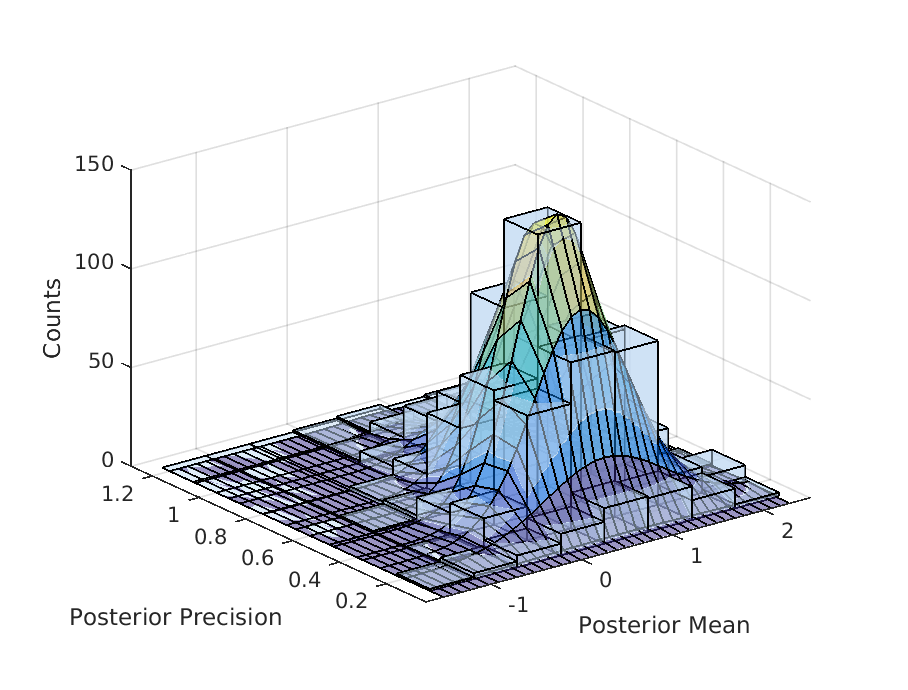
\includegraphics[width=0.5\textwidth]{surf.eps}
\caption{Joint histogram of 1000 samples from ABC. Confidence level set at $10\%$.}
\label{surf}
\end{figure}
\end{frame}

\begin{frame}
\frametitle{Normal-gamma prior, Normal likelihood}
\begin{figure}
\centering
\begin{subfigure}
\centering
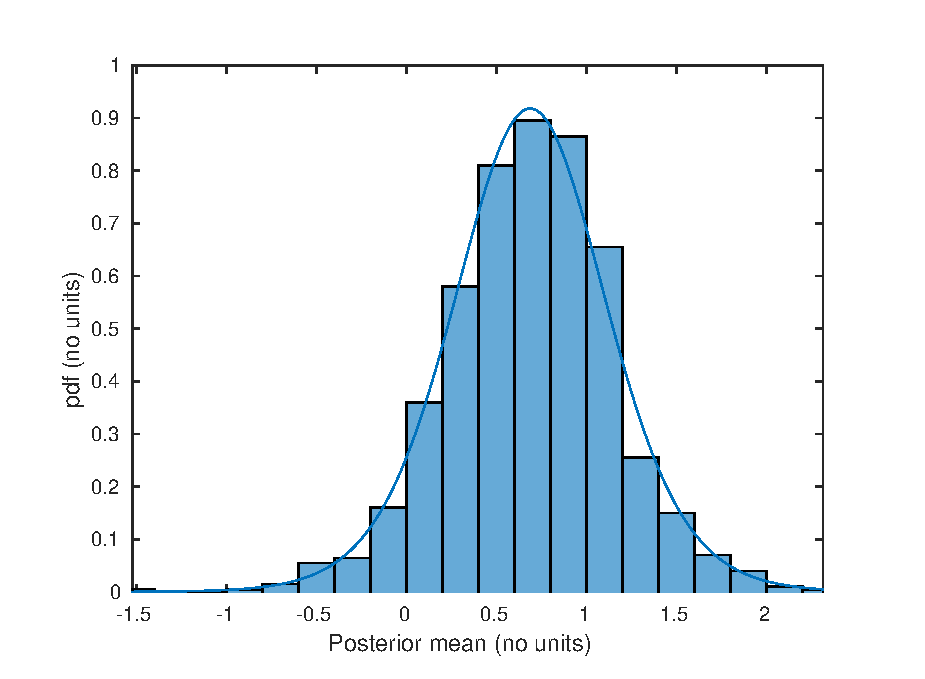
\includegraphics[width=0.45\textwidth]{mean.eps}
\end{subfigure}
\begin{subfigure}
\centering
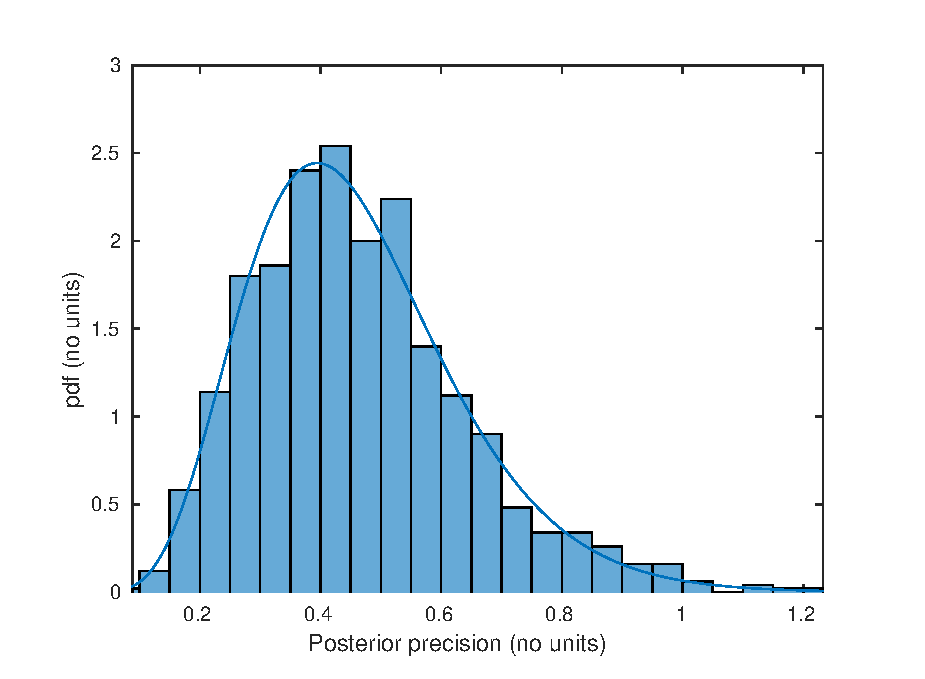
\includegraphics[width=0.45\textwidth]{precision.eps}
\end{subfigure}
\caption{Marginal histogram of 100- samples from ABC. Confidence level set at $10\%$.}
\end{figure}
\end{frame}

\begin{frame}
\frametitle{Normal-gamma prior, Normal likelihood}
\begin{figure}
\centering
\begin{subfigure}
\centering
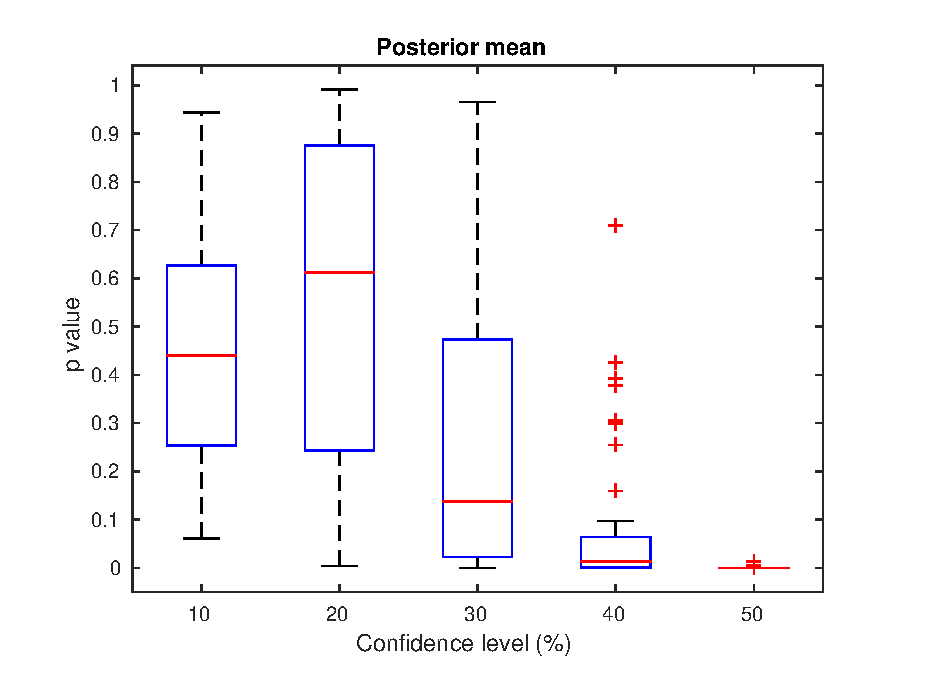
\includegraphics[width=0.45\textwidth]{pvalue_mean.eps}
\end{subfigure}
\begin{subfigure}
\centering
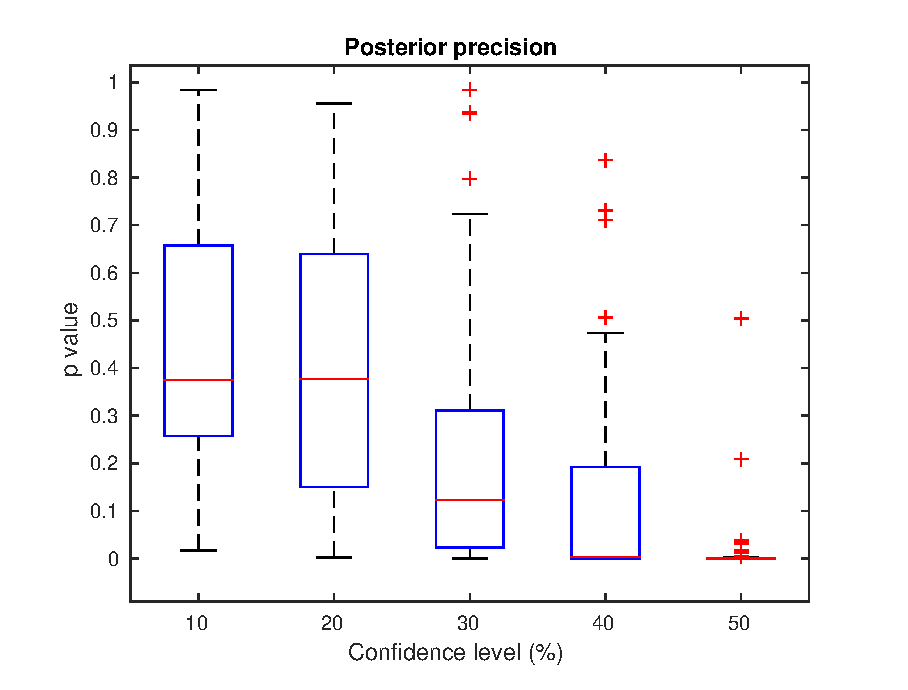
\includegraphics[width=0.45\textwidth]{pvalue_precision.eps}
\end{subfigure}
\caption{$p$ values for the $\chi^2$ goodness of fit test. The test was conducted 50 times with different observations.}
\end{figure}
\end{frame}

\begin{frame}
\frametitle{Normal-gamma prior, Normal likelihood}
\begin{figure}
\centering
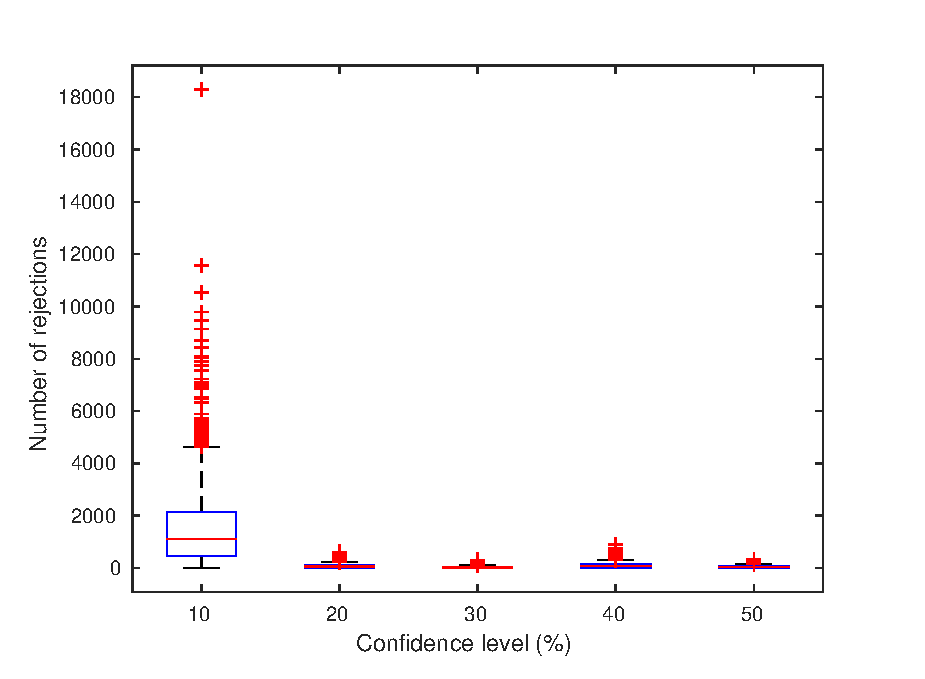
\includegraphics[width=0.45\textwidth]{rejections.eps}
\caption{Rejections per accepted sample}
\end{figure}
\end{frame}

\begin{frame}
\begin{itemize}
\item Threshold not too big, not too small.
\item Ideally distance through sufficient statistics.
\item Posterior can be unknown.
\item Unable to simulate from improper priors.
\end{itemize}
\end{frame}

\end{document}
